\documentclass[12pt,a4]{article}
%%%%%%%%%%%%%%%%%%%%%%%%%%%%%%%%%%%%%%%%%%%%%%%%%%%%%%%%%%%%%%%%%%%%%%
\usepackage{amsmath,amsthm}
\usepackage{bm}
\usepackage{amsfonts}
\usepackage{amssymb}
\usepackage[normalem]{ulem}
\usepackage{enumerate}
\usepackage{graphicx}%
\usepackage{datetime,verbatim}
\usepackage{cite}
\usepackage{hyperref}
\usepackage{listings}

%%%%%%%%%%%%%%%%%%%%%    page setup   %%%%%%%%%%%%%%%%%%%%%%%%%%%%%%%

\textheight=245truemm \textwidth=160truemm \hoffset=-8truemm
\voffset=-23truemm

%%%%%%%%%%%%%%%%%%%%%%%%%%%%%%%%%%%%%%%%%%%%%%%%%%%%%%%%%%%%%%%%%%%%%
\usepackage{fancyhdr}
\pagestyle{fancy}
\lhead{{\sf\scriptsize }}
\rhead{{\sf\scriptsize Winter~2020}}
\chead{{\sf\scriptsize Linear Algebra: Course Project @  DS master programme at UCU}}

\lfoot{}
\rfoot{}
\cfoot{\rm\thepage}

%%%%%%%%%%%%%%%%%%%%%%%%%%%%%%%%%%%%%%%%%%%%%%%%%%%%%%%%%%%%%%%%%%%%%


%%%%%%%%%%%%%%%%%%%%%%%%%%%%%%%%%%%%%%%%%%%%%%%%%%%%%%%%%%%%%%%%%%%%%


%%%%%%%%%%%%%%%   matrix extension  %%%%%%%%
\makeatletter
\renewcommand*\env@matrix[1][*\c@MaxMatrixCols c]{%
	\hskip -\arraycolsep
	\let\@ifnextchar\new@ifnextchar
	\array{#1}}
\makeatother
%%%%%%%%%%%%%%%%%%%%%%%%%%%%%%%%%%%%%%%%%%%%

\newenvironment{proofNoQED}[1]{\smallskip\noindent{\it Proof #1.}\ \rm}
{\hfill \smallskip}
\newcommand{\ProofNoQED}[1]{\smallskip\noindent{\it Proof} #1\ \hfill\smallskip}
%\renewcommand{\qedsymbol}{\text{$\square$}}

\newtheorem{problem}{Problem}

%%%%%%%%%%%%%%%%%%%%%%%%%%%%%%%%%%%%%%%%%%%%%%%%%%%%%%%%%%%%%%%%%%%%%

%%%%%%%%%%%%%%%%%%%%%%%%%%%%%   Definitions       %%%%%%%

\newcommand\ls{\operatorname{ls}}
\newcommand\rank{\operatorname{rank}}
\newcommand{\trace}{\operatorname{tr}}
\newcommand\grad{\operatorname{grad}}


\newcommand{\ov}{\overline}
\newcommand{\wt}{\widetilde}

\newcommand{\bla}{\bm{\lambda}}


\newcommand{\bN}{{\mathbb N}}
\newcommand{\bR}{{\mathbb R}}
\newcommand{\bZ}{{\mathbb Z}}

\newcommand{\ba}{{\mathbf a}}
\newcommand{\bb}{{\mathbf b}}
\newcommand{\bff}{{\mathbf f}}

\newcommand{\bu}{{\mathbf u}}
\newcommand{\bv}{{\mathbf v}}
\newcommand{\bp}{{\mathbf p}}
\newcommand{\bq}{{\mathbf q}}
\newcommand{\br}{{\mathbf r}}
\newcommand{\bx}{{\mathbf x}}
\newcommand{\by}{{\mathbf y}}
\newcommand{\bw}{{\mathbf w}}

\newcommand{\cB}{{\mathcal B}}
\newcommand{\cF}{{\mathcal F}}
\newcommand{\cG}{{\mathcal G}}
\newcommand{\cN}{{\mathcal N}}
\newcommand{\cP}{{\mathcal P}}
\newcommand{\cT}{{\mathcal T}}

%%%%%%%%%%%%%%%%%%%%%%%%%%%%%%%%%%%%%%%%%%%%%%%%%%%%%%%%%%%%%%%%%%%%%


\begin{document}

\begin{center}
  \Huge\bf{Keystroke Dynamics in User Identification}
\end{center}

\begin{center}
	Sevil Smailova, Kateryna Ruskykh and Volodymyr Byno
\end{center}

\large\textbf{Abstract}
\bigskip

\normalsize
In this course project, we will study keystroke dynamics as a method to identify people, using their typing rhythms. We use z-score and KNN methods that perform well on tasks of people authentication based on small text inputs, to recognize identity of a person, using her predefined (re-typed) large text input. We verify how well unconstrained free text typing patterns of a person help to identify her if we know how this person re-types the same text input. We also compare performance of z-score and KNN methods for the identification tasks.

\bigskip

\large\textbf{Introduction}
\bigskip

\normalsize
Keystroke dynamics (KD) uses the natural rhythm of user typing to identify , authenticate a person, constantly monitor his/her identity or even classify a person.  While physiological biometrics (finger scan, iris scan, retina scan, hand scan, and facial scan) give very good precision, these methods are quite costly for identification and authentication purposes. Keystroke dynamics is less costly, unobtrusive and a relatively accurate method.

KD can be used as an additional authentication step to check if the password is being entered by the right person, what can help against fraud or cheating. Thus, in 2005 the Bank of Ireland added the keystroke dynamics algorithms to the user's authentication process and other banks followed \cite{usman1970strengthening}. KD is a good tool to constantly monitor a typing person's identity that is of great importance for online education institutions and online testing/exams. Cheating and manipulations must be eliminated to certify students and prove their competence. Finally, the most recent use is creating a user's profile and detection of emotions/diseases based on his/her typing patterns.

Research on keystroke dynamics has gained pace since 2003, many simple and more sophisticated methods were applied, although the  European standard for access-control systems of a false-alarm rate of less than 1\%, with a miss rate of less than 0.001\%, to our knowledge, has not been achieved. Moreover, there is less research on free/large texts compared to short inputs (passwords, usernames) and very few (if any) on difference in typing patterns for free (unconstrained) texts and predefined texts inputs. Also, the majority of KD papers focus on authentication goals rather than identification (recognizing a typing person), leaving this area under-researched.

In this report we use two simple statistical and machine learning algorithms, Z-score and KNN, for person identification based on an open dataset of large free and predefined texts. Our goal is to check how  the methods and features that work well on small inputs (passwords, usernames) perform on larger-size inputs and free texts.

\bigskip
\large\textbf{Research Question and Hypotheses}
\bigskip

\normalsize
\textbf{Research Question:} How accurately we can define a person's identity with z-score and KNN algorithms, using a large pre-defined and free text inputs? \\

\textbf{Hypothesis 1}: Z-score and KNN help to identify a user of large text inputs, but accuracy is smaller compared to small inputs. \\

\textbf{Hypothesis 2}: Free (unconstrained) text inputs can help to identify the identity of a person, who typed a predefined text input.

\bigskip

\large\textbf{Literature Review}
\bigskip

\normalsize
The earliest start of significant keystroke dynamics (KD) research dates back to late 1970s and early 1980s \cite{Teh:2013}, \cite{Liakat:2017}, \cite{killourhy2009comparing}. After 2003 the number of papers on KD increased significantly, indicating a high interest in the topic \cite{Teh:2013}. Indeed, google scholar returns 62 publications on KD in 2000, 103 in 2003, 232 in 2005 and 995 in 2019, implying a 16 times boost in number of publications between 2000 and 2019. The research on KD varies a lot in their topics (verification vs identification), platform (desktop vs mobile/ tablet), data-collection strategies (size, input type), feature sets, static or dynamic character etc.

The KD publications that focus on verification (the process of proving a validity of claimed identity) outnumber identification (the processes of recognizing a presented identity), as the latter is time-consuming and requires more processing capacities \cite{Teh:2013}, \cite{banerjee2014_emnlp}. Most of the publications on KD do their research on a relatively small dataset involving 21-50 people, typically scholars or students from the researchers’ institution capacities [1,6]. According to the research of 2016, 40 \% out of 88 of the KD publications reviewed involved 21-50 participants, while the reviews of up to 20 and over 100 people accounted for 24 \% each \cite{Liakat:2017}. In recent years KD researchers have more opportunities to expand the number of participants involved and size of collected datasets.

The KD research can deal with a short-text input (password, username, short text phrase, digits) or long-text (over 100 words). The latter can be unconstrained free-text that is often used in continuous authentication systems - systems that dynamically check users’ identities while they are typing. In the review of 2016 the short-text and digits publications account for 60 \% out of 88, while long-text publications take a 22 \% share \cite{Liakat:2017}.

The most common features that are used in the KD research are timing measures: dwell time (the time interval between press of a key and its release) and flight time (the time interval between releasing one key and pressing the other). Most of the researchers use di-graphs: timing measures between two consecutive keys, but n-graphs (three or more keys) can be also used). Other features used by researchers are mouse position / movement, pressure, text correction features, frequencies of errors, average typing speed / acceleration, etc.

There are also a variety of methods to analyze keystroke data that can be grouped as statistical methods (mean, deviations, t-tests, outlier count (z-score), chi-squared, Bayesian modelling, logistic regression, etc.), distance measures (Euclidean, Manhattan, Mahalanobis, Chebyshev, other distance-based measures) and machine learning methods (Artificial Neural Networks, decision trees, KNN, random forest, SVM, etc.). However, it is hard to compare performance and accuracy metrics of different methods, as different authors use different databases, sets of features, model parameters, input types, modes (static or dynamic), etc. There is a benchmark research of Killourhy and Maxion that dates back to 2009, where the authors collect (and make it public) a dataset and compare 14 different methods (detectors) in similar settings \cite{killourhy2009comparing}.

Killourhy and Maxion selected  a 10-character password “.tie5Roanl” , recruited 51 people who were asked to type the password 400 times in 8 sessions. The feature set used included  Keydown-Keydown time between consecutive keys (in some publications referred to as latency), dwell time and flight time. And the authors used 14 algorithms (detectors) that had produced promising results in research of other scientists for authentication of potential impostors. The best-performing algorithms are defined, using two metrics: equal-error rate / ERR (a threshold to discriminate a potential impostor is chosen to have equal miss and false alarm rates) and zero-miss false-alarm rate / ZMFAR (a threshold is selected in a way that a miss rate is 0 and false alarm rate is minimized). We list the top 5 using these 2 metrics in the table below:

\begin{center}

\begin{tabular*}{\textwidth}{l @{\extracolsep{\fill}} lllll}

\hline
 & \textbf{Detector} & \textbf{EER} & & \textbf{Detector} & \textbf{ZMFAR} \\
 \hline
1. & Manhattan (scaled) & 0.096 & 1. & Nearest Neighbor (Mahalanobis) & 0.468 \\
\hline
2. & Nearest Neighbor (Mahalanobis) & 0.100 & 2. & Mahalanobis & 0.482 \\
\hline
3. & Outlier Count (z-score) & 0.102 & 3. & Mahalanobis (normed) & 0.482 \\

\hline
4. & SVM (one-class) & 0.102 & 4. & SVM (one-class) & 0.504 \\
\hline
5. & Mahalanobis & 0.110 & 5. & Manhattan (scaled) & 0.601 \\
\hline
\end{tabular*}
\textbf{Table 1:} The best algorithms / detectors for KD authentication by Killourhy and Maxion
\end{center}

Interestingly, the simplest distance algorithms show the best results according to Killourhy and Maxion. There is also a good score for a machine learning SVM detector and a statistical z-score method. Neural Networks (standard) and k-means give the worst results out of 14 algorithms tested.

Other researchers have been questioning the results of Killourhy and Maxion, testing algorithms on different text inputs (long-text) and datasets (unconstrained datasets of free text). Overall, statistical and distance methods have been losing popularity, while machine learning approaches are gaining pace in the modern times \cite{Liakat:2017}. Support Vector Machine (SVM) is  considered by some researchers as a prevailing machine learning classification approach that produces good results and has reasonable complexity \cite{Liakat:2017}, \cite{raul2020comprehensive}.

Concerning identification research, scholars also show quite good accuracy (over 90\%)\cite{banerjee2012biometric}, however, the number of subjects are usually small - below 35 people.

\bigskip
\large\textbf{Dataset}
\bigskip

\normalsize
For our work we have chosen the  \href{http://www3.cs.stonybrook.edu/~rbanerjee/project-pages/keystrokes/keystrokes.html}{Keystroke Patterns as Prosody in Digital Writings} data \cite{banerjee2014_emnlp} that contains 3 datasets: \begin{itemize}
	\item \textbf{Restaurant Reviews}: The dataset consists of 1000 unique restoran reviews inputed by 500 unique users
	\item \textbf{Gun Control}: The dataset consists of 800 unique essays on "Gun Control" from 400 unique users
	\item \textbf{Gay Marriage}: The dataset consists of 800 unique essays on "Gay Merriage" topic  from 400 unique users
\end{itemize}.
The datasets were collected for the paper on using keystroke dynamics for
deception detection (recognizing deceptive/fake text) \cite{banerjee2014_emnlp}. The authors collected the data via Amazon Mechanical Turk. The Turkers were asked to write 2 free texts: a truthful (true) and deceptive (fake) texts. There were restaurant reviews, opinions on gay marriages and gun control (stored in three separate datasets). After completing their two review(true and fake), each Turker was asked to copy their own typing: copy1 is a copy of true text and copy2 is a copy of fake text (or vice versa). Therefore, the dataset contains keystroke samples for two free texts and the same re-typed copied texts. We merged all 3 datasets into 1 and used it in our analysis. \\

The authors opened access to their dataset. The typical raw data looks like this:
\bigskip

\begin{text}
	0 MouseUp 0 0;16705 KeyDown 16;17170 KeyDown 16;17200 KeyDown 16;17229 KeyDown 16;17258 KeyDown 16;17287 KeyDown 16;17317 KeyDown 16;17346 KeyDown 16;17375 KeyDown 16;17404 KeyDown 16;17433 KeyDown 16;17463 KeyDown 16;17492 KeyDown 16; ...
\end{text}
\bigskip

We used the raw data to extract the timing features described in the next section.

\bigskip
\large\textbf{Web Application}
\bigskip

\normalsize
In order to collect our own data, we've created and deployed a \href{https://powerful-spire-05992.herokuapp.com/}{web application}. It collects keystroke metadata upon user enters the suggested text. It also checks if the text is valid and responds if user made a mistake.

\begin{center}
	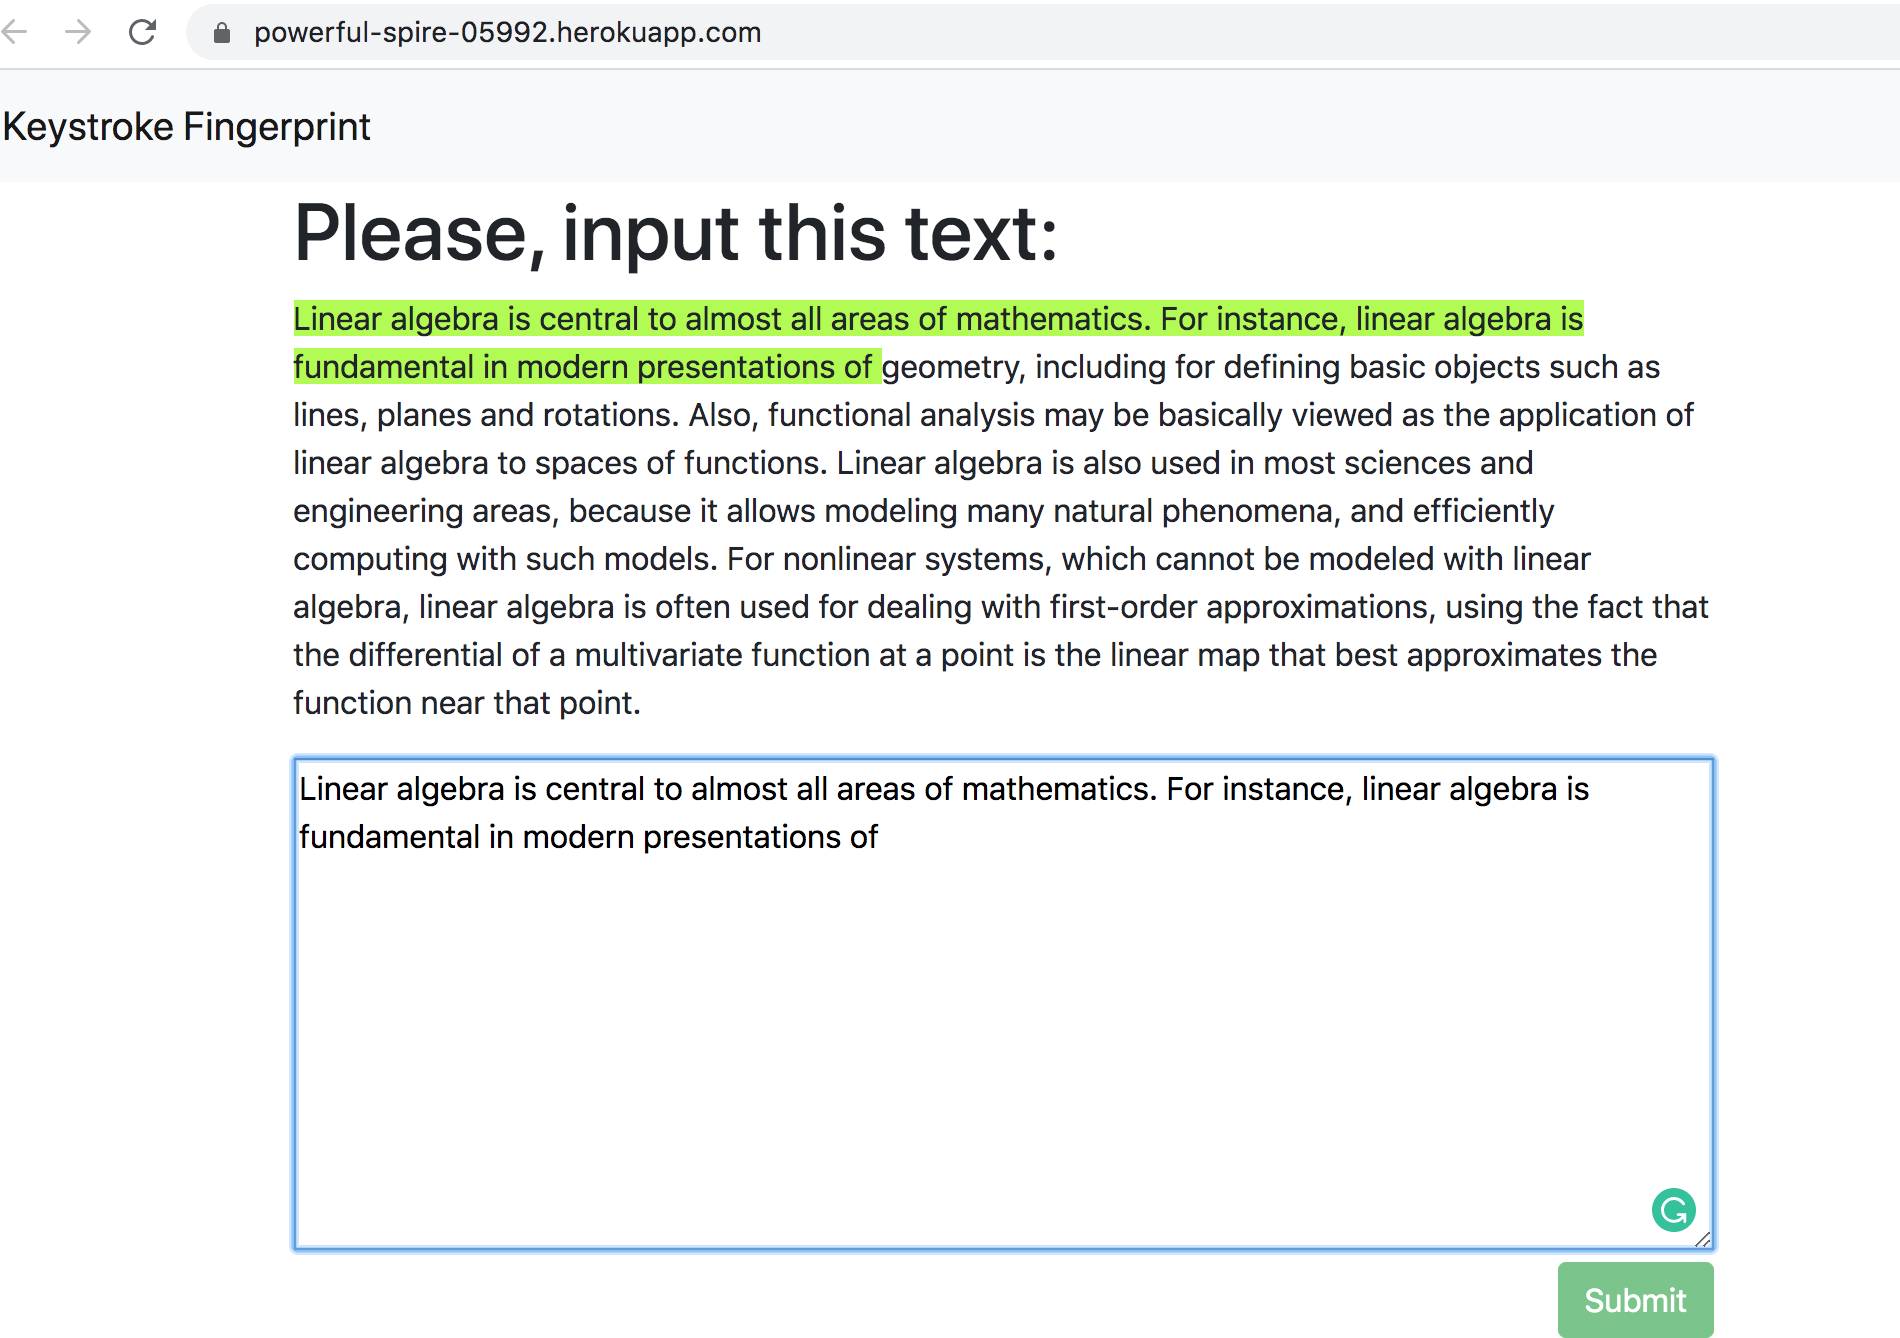
\includegraphics[width=0.9\linewidth]{images/web-app.png}
	\label{fig:web-app.png}
\end{center}
The user has to login to start to enter the text. After a user submits entered text, the keystroke metadata is saved in the database.
Predefined admin users could download the keystroke data of all users. Although the keystroke data is anonymized, it does not contain the user's login/email or other personal data. It is mapped to self-generated UUID which is unique for each user. So, it is possible to distinguish the keystroke patterns and use this data for model learning.

At the current moment, we've collected 28 text inputs from 17 unique users.

\bigskip
\large\textbf{Features Extraction}
\bigskip

\normalsize

The main problem we have encountered with is the proper feature selection. The user can be identified by his typing behavior. This behavior can be expressed by the timing of different key-presses. The number of keys that include a single keypress or keypress of two successive keys increases the amount of features that we can use in modelling. So we tried to use several set of them in order to check their influence on results. \\

In our work we used: \textbf{dwell time} (the latency between pressing and releasing a key) and \textbf{flight time} (in our case a time between key downs of two successive keys(\textbf{digraphs})). In our dataset we have 105 dwell times of unique keys/letter and 3099 flight times of unique digraphs, jointly 3204 features. Many of the features are not relevant, thus, we use the approach recommended in \cite{tappert2012keystroke}. \\

For z-score method we used the dwell time of the 8 most frequent keys/letters, in our case:
'E', 'A', 'R', 'I', 'O', 'T', 'N', 'S' and 'space'. And the flight time of the 12 most frequent digraphs, in our case: 'S\_space', 'space\_A', 'D\_space', 'E\_space', 'space\_T', 'backspace\_backspace', 'T\_H', 'H\_E', 'A\_N', 'T\_space', 'R\_E', 'I\_N.
To remove outliers we used approaches Interquartile Range (IQR) method (for z-score identifier) and standard deviation method (for KNN). According to IQR we removed data points below $Q1 – 1.5 \times IQR$ or above $Q3 + 1.5 \times IQR$, where Q1 and Q3 are the first and third quantities, IQR = Q3-Q1. \\

As the starting point we used the dwell time of the 8 most frequent keys/letters, in our case:
'E', 'A', 'R', 'I', 'O', 'T', 'N', 'S' and 'space'. And the flight time of the 12 most frequent digraphs, in our case: 'S\_space', 'space\_A', 'D\_space', 'E\_space', 'space\_T', 'backspace\_backspace', 'T\_H', 'H\_E', 'A\_N', 'T\_space', 'R\_E', 'I\_N. \\


\bigskip
\large\textbf{Methodology }
\bigskip

\medskip
\small\textbf{Z-SCORE Identification}
\medskip

\normalsize

Killourhy and Maxion \cite{killourhy2009comparing} used Outlier Count (z-score) detector to authenticate impostors, and this simple statistical method displayed quite good results: the thirds lowest equal-error rate among the 14 detectors (see table above).  The idea of the method by Kollourhy and Maxion is to calculate mean vector $m_i$ and standard deviation vector $s_i$ for each feature of each known subject at the training phase. Then in the test phase the authors calculate the absolute z-score of each feature $i$ of the test vector: $|x_i-m_i|/s_i$. The anomaly score is a count how often the calculated z-score exceeds a threshold of 1.96. If the number is large (the authors do not specify how large), a subject is set to be an impostor.

We used the Outlier Count (z-score) method with some modifications for our identification goal. We calculate mean $m$ and standard deviation vectors $std$, that are $k \times 1$ vectors with means and standard deviations of each feature in Copy 1 text for a subset of our subjects in the train phase. In this method the number of features k is equal to 21.
$$
\overline{m} = \frac{1}{n}i^T x
$$
 where $x$ is a $n\times 1$ dimensional time vector of the feature $i$ in the Copy 1 task. $n$ is a count of the $ith$ feature occurrence in the Copy1 text of each subject in the train set. \\
$$
s^2 = \frac{1}{n-1} x^T M x
$$
\\
where M  is an idempotent matrix:
$$
M = I - \frac{1}{n}ii^T
$$

where $x$ is a $n\times 1$ dimensional time vector of the feature $i$ in the Copy 1 task. $n$ is a count of the $ith$ feature occurrence in the Copy1 text of each subject in the train set.\\
\\
In the test phase we calculate z-score, a $n \times m$ matrix. N is a number of features (21 for this method), while m is the maximum occurrence of a feature for a subject in the test phase.
$$
zscore = \frac{|X^{test} - m|}{s}
$$
where $X^{test}$ is a $n\times m$ matrix of the $ith$ feature in the texts of subjects in the test set. $M$ is equal to the length of the largest feature vector for a given subject in the test phase. \\
\\
In the next step we construct Zcount matrix, that $n \times m$ matrix such that:
$$
zcount_{rule} = \begin{cases} 1, & \mbox{if } zscore \mbox{ $<$ 1.96} \\ 0, & \mbox{ } \mbox{ otherwise} \end{cases}
$$
Next, we need the vector that count relative number of times each feature is accepted (smaller than our threshold). To make $zcount_r$ vector (a $n \times 1$ vector) we sum each row of of the Zcount matrix and divide by the count of 1s in each row.
\\
\\
The closer this $zcount_r$ vector to a vector of ones (i vector), the closer is a tested subject's keyprint style to true subject. To find out this distance we use the Euclidian distance metric:
$$
d = ||zcount_r - i||
$$

The subject and task with the smallest distance is the predicted subject. Accuracy measure is the relative number of times we correctly predict the true subject.\\
\\
\small\textbf{PSEUDOCODE}

\normalsize

\begin{lstlisting}
FOR user in TRAIN_SET:
    true_user = user
    mean(x) <- get the mean vector for the user
    std(x) <- get the std vector for the user
    for user_test in TEST_SET:
        for tasks in [copy1, copy2, true, false]:
            f = get_features(user, taks) <- features matrix of user, task
            Zscore = abs(f-mean(x)/std(x) <- matrix of z scores
            zrule = if (r < threshold) than 1, else 0
            Zcount = Zscore apply zrule
            zcount_result = sum(Zcount by row)/count(1s in each row)
            ones <- vector of 1s
            d = distance_euclidean(zcount_result, ones)
        predicted_user = user with the minimum d
    if predicted_user == true_user:
            accuracy.append(1)
    else:
            accuracy.append(0)

ACCURACY = SUM(accuracy)/len(accuracy)

\end{lstlisting}



\bigskip
\small\textbf{Nearest Neighbour Algorithm on PCA features}
\bigskip

\normalsize

The nearest neighbour detector aims to define the smallest distance between the the feature vectors. The input data is considered to be a set of most spread digraphs and letters per each user.  The accuracy of the method is calculated by the dividing number of predicted users over all number of users.

The distance that is used to find the nearest neighbour is Euclidean Distance:\\


$$
d(a,b) = d(b,a) = \sqrt{\sum_{n=1}^{n} (a_i - b_i)^2},
$$\\

where $a, b$ - are the samples of two users, $n$ - the number of features we consider to use to describe the specifics of each  user behavior.\\

So in order to identify the user we need to calculate the distances between feature vectors of all users and find the smallest distance. This smallest distance will show us the most similar user to the one we wont to identify. We take the number of neighbors equal to 1 because we have only one observation in the test sample that is responsible for the entire class it belongs to.

The problem with big amount of features was resolved by applying the PCA that cover the 90\% of the variance and left only 9 input variables.


\newpage
\bigskip
\large\textbf{Results}
\bigskip

\medskip
\small\textbf{Z-SCORE Identification}
\medskip

\normalsize

We tested our Z-score identification methodology on 3 randomly selected subsets of subjects: 20, 50 and 100 subjects. We obtained the corresponding accuracy metrics of 80\%, 68\% and 57\%. The prevailing share of the correctly identified subjects were recognized by copy2 text: within 57 \% of correctly selected subjects, 60 \% where recognized by copy2 texts, 17 \% by true reviews and 21 \% by fake reviews. This results prove that keystroke patterns for free text and pre-defined re-typed text are different, as the algorithm recognized primarily not the same texts with the same features (`copy1` text of a user is the same with either true or fake reviews), but the re-typing keyprint pattern of a user for a different text.

As expected, accuracy scores are relatively small. We had a small text dataset for a user: our model is trained on 1 text sample with no repetitions. Moreover, long texts (as well as free text) requires more sophisticated feature extraction techniques, as simple digraphs work good for passwords, usernames and digits, while in long text not only digraphs, but their positioning is potentially important. Moreover, not all features are equally important - some of them are more discriminating than the other, while in our z-score algorithm all features are treated equally, also disregarding how often they appear in the text of a given subject.


\medskip
\small\textbf{KNN with PCA Identification}
\medskip

\normalsize

Performance of the KNN method was measured by using 3 randomly chosen sub-samples: 100, 500 and 700 unique users. The corresponding accuracy's equal to 83\%, 67\% and 64\%. The training sample is a combination of a "true", "false" and "copy 2" texts. The test sample is contains users keystrokes from "copy 2" tests. We can see that the number of observation significantly influence on the ability to distinguish between the user tying pattern by which they can be recognized. As was suggested above, the increasing the number of observations we can add more information about the distribution of the keystrokes.

\bibliography{keystroke_dynamics}{}
\bibliographystyle{plain}
\end{document}
